\chapter*{Appendix}
\addcontentsline{toc}{chapter}{Appendix}

\section*{Haskell Symposium 2021 Paper and Reviews} \label{symposiumfeedback}

This section includes the anonymised Haskell Symposium 2021 paper, submitted for the early track, as well as the feedback received from the reviewers.

\subsection*{Review A}

\subsubsection*{Overall merit}

3. Weak accept

\subsubsection*{Reviewer expertise}

4. Expert

\subsubsection*{Paper summary}

The paper describes a type level EDSL for describing chess games in Haskell, using the type system to guarantee that the games are valid according to the rules of chess. It highlights some of the limitations of type level programming in Haskell and proposes some workarounds.

\subsubsection*{Comments for author}

This is an interesting paper, which tests the limits of type level programming in Haskell on a fairly complex problem, representing the rules of Chess. It relies on First Class type families, a technique (or perhaps a workaround) which allows partial application of type level functions.

I think the real value of this paper is in showing the limits of type level programming in Haskell and identifying where it can be improved both in terms of type checker performance, and in usability in general. It always seems that, no matter how much more gets added to type level programming in GHC, we always end up needing a little bit more! This isn't a criticism of the paper - in fact I think the paper does a good job of demonstrating that.

The end result is an impressive technical achievement, but I think the evaluation is quite limited, and there isn't much (if any) discussion of how this kind of type level programming would be incorporated into a real application, e.g. a chess playing program. What can we learn from this work about type level programming in Haskell in general? Is it a good idea? We see the end product, but there's little discussion of how hard it was to arrive at the result, and how it might compares with type level programming in other systems. Does the type checker help you during development, e.g. through typed holes? What kind of error messages do you get? On performance, would systems designed from the start for type level programming be more efficient for type checking these problems? We see the performance in GHC in section 5, and there is some useful discussion here, but it's only about GHC itself. Perhaps the conclusion should be that Haskell isn't going to be suitable for this type of type level program, or perhaps it's just a fundamentally hard thing to do at the type level, or perhaps this suggests GHC needs a new approach to type level computation. It's hard to say without more detailed comparisons to related work to learn what is possible, but it looks to me like the programming involved isn't that complex and the difficulty is in making it work at the type level.

I did wonder if all the details in section 3 were necessary for understanding the EDSL - once we have the idea of how to query the board at the type level, is there much more to say, even about the special movement rules? If this was more concise, there'd be more space for a detailed evaluation.

Still, overall I would like to see this accepted - it's valuable to see how people are pushing the limits of type level programming in Haskell - but I think it really needs more discussion about how it relates to tackling similar problems in other dependently typed systems.

A few other more specific things:

100 - is the intention of Chesskell just to describe games, or would we expect to use it as part of a larger project, say a chess implementation with some verification that it's following the rules of chess properly? Without a bit of context, one might wonder why doing this at the type level is any better than writing an ordinary program that returns a Bool!

111 - is this really a contribution of this paper? It's useful tutorial material to put the rest into context, but I'm not sure it belongs as a contribution. Is there something you can cite here?

189 - this seems a neat workaround for a limitation of type families although it does seem to rely on writing type families this way in the first place. Might this suggest that they should be implemented differently inside GHC?

234 - again, it seems to be a limitation of type level programming in Haskell that it requires reimplementing standard library functions. Is this a limitation of other systems too?

258 - would we expect first class families to have corresponding value level functions? I guess we would if this was part of a larger chess playing program.

340 extra word "we use encode this" (aside: nice to see an actual use for vectors beyond an introductory example!)

793 - are these the actual error messages? If you, how do you set that up? It seems important for the ergonomics of the system as a whole.

970 - I think these measurements (memory usage and compile times) are sufficiently important to warrant some more detailed evaluation - can you perhaps tabulate a few games and the resources required to check them?

1321 - I'm surprised to see so few references given how much work there has been in type level programming in recent years, not only in Haskell but in other systems. How does it relate to other systems, especially those with full dependent types, e.g. Idris, Agda, or even Coq? Would using these systems have taken less effort, and does that suggest it's worth pursuing full dependent types in Haskell, or not? It would be good to discuss this in related work. There's also related work just in the history of building up type level programming in Haskell, one relevant example being "Hasochism" from Haskell 2013.

\subsection*{Review B}

\subsubsection*{Overall merit}

2. Weak reject

\subsubsection*{Reviewer expertise}

4. Expert

\subsubsection*{Paper summary}

The paper presents an EDSL for chess games which is strongly based on type-level programming. Each game is specified as a sequence of moves using either a shorthand or a longhand notation. The EDSL prevents the occurrence of invalid moves by checking their validity against the chess rules; this checking is fully performed at the type level. This is the result of the data type promotion of all the ingredients that conform a chess game (players, pieces and board), which are given by certain datatype representations, and the type-level implementation of the operations that evaluate (and check) the moves.

In addition to the strong use of type-level programming, the EDSL presents other interesting aspects in its design, like the use of the First Class Families technique (a sort of deep embedding to model higer order type-level functions) for the implementation of the type-level functions or the use of flat combinators in the sense introduced by Okasaki for the shorthand chess notation.

\subsubsection*{Comments for author}

The paper is interesting to read. I found it well-written and clear in its exposition.

However, considering the kind of application that the EDSL implements (essentially an analyzer that checks the well-formedness of chess games), my main concern is with the usefulness and suitability of the type-level solution presented. In this sense, the authors should argue why in this case they consider that a full type-level solution is more beneficial than a more standard one worked out at the value level.

I agree with the advantages of using type-level programming. It is a powerful tool that assists in the development of more robust programs, but on the other hand, its usefulness depends on each case. In the particular case of this EDSL, I really don't see the advantage of performing the verification of the games at the type level. Since the goal is to simply check their validity, why not to simply implement that checking at the value level (using the same design of operations and checks that was used for the type level). In particular, this would avoid all the difficulties encountered during compilation.

In my opinion, in the present state, the paper contribution is based more on the results obtained from applying the stress test (resulting from the solution developed) to the type system than on the solution itself.

Finally, I mention another approach to higher order type level programming in Haskell that perhaps may help in this case: Higher-Order Type-Level Programming in Haskell, Kiss et.al., ICFP 2019.

Comments/Typos:

\begin{itemize}
      \item Page 2, 161
            I think it would equally work if you define
            type Exp (a :: Type) = Type
            instead of
            type Exp (a :: Type) = a -> Type

      \item Page 2, 189 (in the definition of Map)
            replace "f a" by "[a]"
            replace "f b" by "[b]"

      \item Page 3, 291
            an type -> a type

      \item Page 6, 561
            they have -> it has

      \item Page 7, 735-736
            chess functions -> chess function

      \item Page 9, 914
            This the
\end{itemize}

\subsection*{Review C}

\subsubsection*{Overall merit}

3. Weak accept

\subsubsection*{Reviewer expertise}

3. Knowledgeable

\subsubsection*{Paper summary}

This paper used type level programming to implement the rules of Chess and a DSL for describing chess games. The paper does push the use of type level programming to unusual limits, with games being limited to approximately 12 moves by each player. The paper makes extensive usage of existing and known techniques, but at a scale not usually attempted.

\subsubsection*{Comments for author}

This was a fun paper to read, and quite well written. I have a few suggestions for improvement.

Providing an overview of a known technique is not a contribution, as such. I'd move this bullet into its own subsubsection*, then say something like: using this technique allows use to make the following three contributions…

For the example on page 2 that fails, add a comment to highlight this in the code.

Section 3. For the model, you should compare it with an actual Haskell implementation, using the same algorithms and data structures. This should be syntactically straightforward.

It is not clear how much we learn from implementing En Passant, except saying the game is chess complete.

I loved the DSL(s) for replacing pgn, and the DSL for fen. Neat! I'm not sure why you had two languages for png, though. What did one buy over other the other, except slight syntactical form.

Why not just use FEN?

Fix the widow on page 8/9.

The fact this stressed the compiler to the tune of 27GB was interesting. I could imagine the example being used when stress testing the compiler's type checker.

The related work seems unbalanced. Haskell has been used for Chess before.

I disagree about having tools for profiling type-level programing, such as these. Stress what we have, but why would we use a type-level system, when we can use a value-level system for actually doing evaluation?

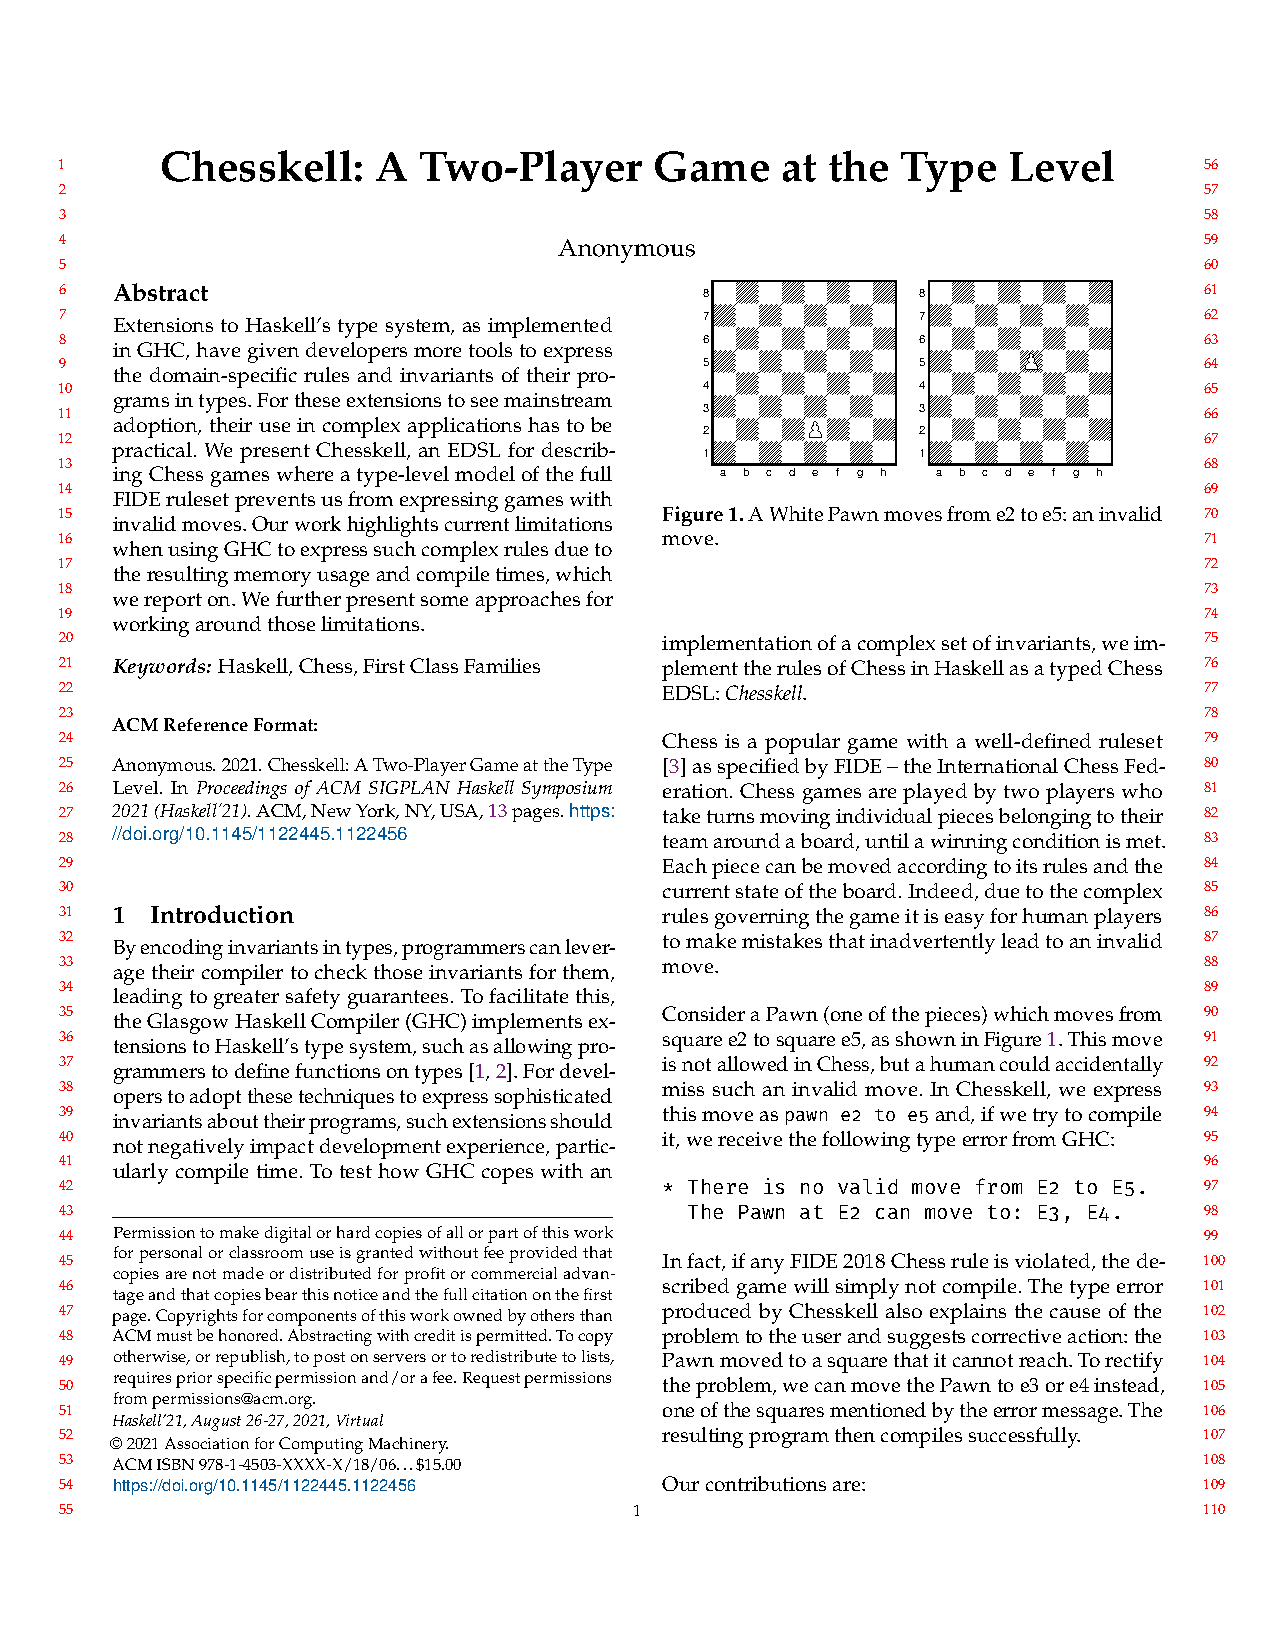
\includepdf[pages=-]{paper.pdf}